\documentclass[11pt,a4paper, d]{scrartcl}
    \usepackage[scaled]{helvet}
    \usepackage{fancyhdr}
    \usepackage{amsmath}
\usepackage{amsthm}
\usepackage{amssymb}
\usepackage{amsfonts}
    \usepackage[breakable]{tcolorbox}
    \usepackage{parskip} % Stop auto-indenting (to mimic markdown behaviour)
    
    \usepackage{iftex}
    \ifPDFTeX
    	\usepackage[T1]{fontenc}
    	\usepackage{mathpazo}
    \else
    	\usepackage{fontspec}
    \fi

    % Basic figure setup, for now with no caption control since it's done
    % automatically by Pandoc (which extracts ![](path) syntax from Markdown).
    \usepackage{graphicx}
    % Maintain compatibility with old templates. Remove in nbconvert 6.0
    \let\Oldincludegraphics\includegraphics
    % Ensure that by default, figures have no caption (until we provide a
    % proper Figure object with a Caption API and a way to capture that
    % in the conversion process - todo).
    \usepackage{caption}
    \DeclareCaptionFormat{nocaption}{}
    \captionsetup{format=nocaption,aboveskip=0pt,belowskip=0pt}

    \usepackage[Export]{adjustbox} % Used to constrain images to a maximum size
    \adjustboxset{max size={0.9\linewidth}{0.9\paperheight}}
    \usepackage{float}
    \floatplacement{figure}{H} % forces figures to be placed at the correct location
    \usepackage{xcolor} % Allow colors to be defined
    \usepackage{enumerate} % Needed for markdown enumerations to work
    \usepackage{geometry} % Used to adjust the document margins
    \usepackage{amsmath} % Equations
    \usepackage{amssymb} % Equations
    \usepackage{textcomp} % defines textquotesingle
    % Hack from http://tex.stackexchange.com/a/47451/13684:
    \AtBeginDocument{%
        \def\PYZsq{\textquotesingle}% Upright quotes in Pygmentized code
    }
    \usepackage{upquote} % Upright quotes for verbatim code
    \usepackage{eurosym} % defines \euro
    \usepackage[mathletters]{ucs} % Extended unicode (utf-8) support
    \usepackage{fancyvrb} % verbatim replacement that allows latex
    \usepackage{grffile} % extends the file name processing of package graphics 
                         % to support a larger range
    \makeatletter % fix for grffile with XeLaTeX
    \def\Gread@@xetex#1{%
      \IfFileExists{"\Gin@base".bb}%
      {\Gread@eps{\Gin@base.bb}}%
      {\Gread@@xetex@aux#1}%
    }
    \makeatother
\renewcommand*\familydefault{\sfdefault}
    % The hyperref package gives us a pdf with properly built
    % internal navigation ('pdf bookmarks' for the table of contents,
    % internal cross-reference links, web links for URLs, etc.)
    \usepackage{hyperref}
    % The default LaTeX title has an obnoxious amount of whitespace. By default,
    % titling removes some of it. It also provides customization options.
    \usepackage{titling}
    \usepackage{longtable} % longtable support required by pandoc >1.10
    \usepackage{booktabs}  % table support for pandoc > 1.12.2
    \usepackage[inline]{enumitem} % IRkernel/repr support (it uses the enumerate* environment)
    \usepackage[normalem]{ulem} % ulem is needed to support strikethroughs (\sout)
                                % normalem makes italics be italics, not underlines
    \usepackage{mathrsfs}
    

    
    % Colors for the hyperref package
    \definecolor{urlcolor}{rgb}{0,.145,.698}
    \definecolor{linkcolor}{rgb}{.71,0.21,0.01}
    \definecolor{citecolor}{rgb}{.12,.54,.11}

    % ANSI colors
    \definecolor{ansi-black}{HTML}{3E424D}
    \definecolor{ansi-black-intense}{HTML}{282C36}
    \definecolor{ansi-red}{HTML}{E75C58}
    \definecolor{ansi-red-intense}{HTML}{B22B31}
    \definecolor{ansi-green}{HTML}{00A250}
    \definecolor{ansi-green-intense}{HTML}{007427}
    \definecolor{ansi-yellow}{HTML}{DDB62B}
    \definecolor{ansi-yellow-intense}{HTML}{B27D12}
    \definecolor{ansi-blue}{HTML}{208FFB}
    \definecolor{ansi-blue-intense}{HTML}{0065CA}
    \definecolor{ansi-magenta}{HTML}{D160C4}
    \definecolor{ansi-magenta-intense}{HTML}{A03196}
    \definecolor{ansi-cyan}{HTML}{60C6C8}
    \definecolor{ansi-cyan-intense}{HTML}{258F8F}
    \definecolor{ansi-white}{HTML}{C5C1B4}
    \definecolor{ansi-white-intense}{HTML}{A1A6B2}
    \definecolor{ansi-default-inverse-fg}{HTML}{FFFFFF}
    \definecolor{ansi-default-inverse-bg}{HTML}{000000}

    % commands and environments needed by pandoc snippets
    % extracted from the output of `pandoc -s`
    \providecommand{\tightlist}{%
      \setlength{\itemsep}{0pt}\setlength{\parskip}{0pt}}
    \DefineVerbatimEnvironment{Highlighting}{Verbatim}{commandchars=\\\{\}}
    % Add ',fontsize=\small' for more characters per line
    \newenvironment{Shaded}{}{}
    \newcommand{\KeywordTok}[1]{\textcolor[rgb]{0.00,0.44,0.13}{\textbf{{#1}}}}
    \newcommand{\DataTypeTok}[1]{\textcolor[rgb]{0.56,0.13,0.00}{{#1}}}
    \newcommand{\DecValTok}[1]{\textcolor[rgb]{0.25,0.63,0.44}{{#1}}}
    \newcommand{\BaseNTok}[1]{\textcolor[rgb]{0.25,0.63,0.44}{{#1}}}
    \newcommand{\FloatTok}[1]{\textcolor[rgb]{0.25,0.63,0.44}{{#1}}}
    \newcommand{\CharTok}[1]{\textcolor[rgb]{0.25,0.44,0.63}{{#1}}}
    \newcommand{\StringTok}[1]{\textcolor[rgb]{0.25,0.44,0.63}{{#1}}}
    \newcommand{\CommentTok}[1]{\textcolor[rgb]{0.38,0.63,0.69}{\textit{{#1}}}}
    \newcommand{\OtherTok}[1]{\textcolor[rgb]{0.00,0.44,0.13}{{#1}}}
    \newcommand{\AlertTok}[1]{\textcolor[rgb]{1.00,0.00,0.00}{\textbf{{#1}}}}
    \newcommand{\FunctionTok}[1]{\textcolor[rgb]{0.02,0.16,0.49}{{#1}}}
    \newcommand{\RegionMarkerTok}[1]{{#1}}
    \newcommand{\ErrorTok}[1]{\textcolor[rgb]{1.00,0.00,0.00}{\textbf{{#1}}}}
    \newcommand{\NormalTok}[1]{{#1}}
    
    % Additional commands for more recent versions of Pandoc
    \newcommand{\ConstantTok}[1]{\textcolor[rgb]{0.53,0.00,0.00}{{#1}}}
    \newcommand{\SpecialCharTok}[1]{\textcolor[rgb]{0.25,0.44,0.63}{{#1}}}
    \newcommand{\VerbatimStringTok}[1]{\textcolor[rgb]{0.25,0.44,0.63}{{#1}}}
    \newcommand{\SpecialStringTok}[1]{\textcolor[rgb]{0.73,0.40,0.53}{{#1}}}
    \newcommand{\ImportTok}[1]{{#1}}
    \newcommand{\DocumentationTok}[1]{\textcolor[rgb]{0.73,0.13,0.13}{\textit{{#1}}}}
    \newcommand{\AnnotationTok}[1]{\textcolor[rgb]{0.38,0.63,0.69}{\textbf{\textit{{#1}}}}}
    \newcommand{\CommentVarTok}[1]{\textcolor[rgb]{0.38,0.63,0.69}{\textbf{\textit{{#1}}}}}
    \newcommand{\VariableTok}[1]{\textcolor[rgb]{0.10,0.09,0.49}{{#1}}}
    \newcommand{\ControlFlowTok}[1]{\textcolor[rgb]{0.00,0.44,0.13}{\textbf{{#1}}}}
    \newcommand{\OperatorTok}[1]{\textcolor[rgb]{0.40,0.40,0.40}{{#1}}}
    \newcommand{\BuiltInTok}[1]{{#1}}
    \newcommand{\ExtensionTok}[1]{{#1}}
    \newcommand{\PreprocessorTok}[1]{\textcolor[rgb]{0.74,0.48,0.00}{{#1}}}
    \newcommand{\AttributeTok}[1]{\textcolor[rgb]{0.49,0.56,0.16}{{#1}}}
    \newcommand{\InformationTok}[1]{\textcolor[rgb]{0.38,0.63,0.69}{\textbf{\textit{{#1}}}}}
    \newcommand{\WarningTok}[1]{\textcolor[rgb]{0.38,0.63,0.69}{\textbf{\textit{{#1}}}}}
    
    \graphicspath{{figures/}{MonteCarlo/figures/}{MonteCarlo/}}
    
    % Define a nice break command that doesn't care if a line doesn't already
    % exist.
    \def\br{\hspace*{\fill} \\* }
    % Math Jax compatibility definitions
    \def\gt{>}
    \def\lt{<}
    \let\Oldtex\TeX
    \let\Oldlatex\LaTeX
    \renewcommand{\TeX}{\textrm{\Oldtex}}
    \renewcommand{\LaTeX}{\textrm{\Oldlatex}}
    % Document parameters
    % Document title
  \pagestyle{fancy}
\fancyhf{}
\rhead{\begin{picture}(0,0)(0,0)\put(53,-62){
\includegraphics[height=4cm]{logoR}}\end{picture}}
\lhead{Handout - Monte Carlo Simulations}
\lfoot{File: \jobname, date: \today}
\rfoot{Page \thepage}

\author{Prof. Dr. Raphael Pfaff\\Lehrgebiet Schienenfahrzeugtechnik}
%\begin{picture}(0,0)(0,0)\put(158,390){
\includegraphics[height=4cm]{logoR}}\end{picture}}
\title{Rail Data Science}
\subtitle{Handout - Monte Carlo Simulations}

    
    
    
    
    
% Pygments definitions
\makeatletter
\def\PY@reset{\let\PY@it=\relax \let\PY@bf=\relax%
    \let\PY@ul=\relax \let\PY@tc=\relax%
    \let\PY@bc=\relax \let\PY@ff=\relax}
\def\PY@tok#1{\csname PY@tok@#1\endcsname}
\def\PY@toks#1+{\ifx\relax#1\empty\else%
    \PY@tok{#1}\expandafter\PY@toks\fi}
\def\PY@do#1{\PY@bc{\PY@tc{\PY@ul{%
    \PY@it{\PY@bf{\PY@ff{#1}}}}}}}
\def\PY#1#2{\PY@reset\PY@toks#1+\relax+\PY@do{#2}}

\expandafter\def\csname PY@tok@w\endcsname{\def\PY@tc##1{\textcolor[rgb]{0.73,0.73,0.73}{##1}}}
\expandafter\def\csname PY@tok@c\endcsname{\let\PY@it=\textit\def\PY@tc##1{\textcolor[rgb]{0.25,0.50,0.50}{##1}}}
\expandafter\def\csname PY@tok@cp\endcsname{\def\PY@tc##1{\textcolor[rgb]{0.74,0.48,0.00}{##1}}}
\expandafter\def\csname PY@tok@k\endcsname{\let\PY@bf=\textbf\def\PY@tc##1{\textcolor[rgb]{0.00,0.50,0.00}{##1}}}
\expandafter\def\csname PY@tok@kp\endcsname{\def\PY@tc##1{\textcolor[rgb]{0.00,0.50,0.00}{##1}}}
\expandafter\def\csname PY@tok@kt\endcsname{\def\PY@tc##1{\textcolor[rgb]{0.69,0.00,0.25}{##1}}}
\expandafter\def\csname PY@tok@o\endcsname{\def\PY@tc##1{\textcolor[rgb]{0.40,0.40,0.40}{##1}}}
\expandafter\def\csname PY@tok@ow\endcsname{\let\PY@bf=\textbf\def\PY@tc##1{\textcolor[rgb]{0.67,0.13,1.00}{##1}}}
\expandafter\def\csname PY@tok@nb\endcsname{\def\PY@tc##1{\textcolor[rgb]{0.00,0.50,0.00}{##1}}}
\expandafter\def\csname PY@tok@nf\endcsname{\def\PY@tc##1{\textcolor[rgb]{0.00,0.00,1.00}{##1}}}
\expandafter\def\csname PY@tok@nc\endcsname{\let\PY@bf=\textbf\def\PY@tc##1{\textcolor[rgb]{0.00,0.00,1.00}{##1}}}
\expandafter\def\csname PY@tok@nn\endcsname{\let\PY@bf=\textbf\def\PY@tc##1{\textcolor[rgb]{0.00,0.00,1.00}{##1}}}
\expandafter\def\csname PY@tok@ne\endcsname{\let\PY@bf=\textbf\def\PY@tc##1{\textcolor[rgb]{0.82,0.25,0.23}{##1}}}
\expandafter\def\csname PY@tok@nv\endcsname{\def\PY@tc##1{\textcolor[rgb]{0.10,0.09,0.49}{##1}}}
\expandafter\def\csname PY@tok@no\endcsname{\def\PY@tc##1{\textcolor[rgb]{0.53,0.00,0.00}{##1}}}
\expandafter\def\csname PY@tok@nl\endcsname{\def\PY@tc##1{\textcolor[rgb]{0.63,0.63,0.00}{##1}}}
\expandafter\def\csname PY@tok@ni\endcsname{\let\PY@bf=\textbf\def\PY@tc##1{\textcolor[rgb]{0.60,0.60,0.60}{##1}}}
\expandafter\def\csname PY@tok@na\endcsname{\def\PY@tc##1{\textcolor[rgb]{0.49,0.56,0.16}{##1}}}
\expandafter\def\csname PY@tok@nt\endcsname{\let\PY@bf=\textbf\def\PY@tc##1{\textcolor[rgb]{0.00,0.50,0.00}{##1}}}
\expandafter\def\csname PY@tok@nd\endcsname{\def\PY@tc##1{\textcolor[rgb]{0.67,0.13,1.00}{##1}}}
\expandafter\def\csname PY@tok@s\endcsname{\def\PY@tc##1{\textcolor[rgb]{0.73,0.13,0.13}{##1}}}
\expandafter\def\csname PY@tok@sd\endcsname{\let\PY@it=\textit\def\PY@tc##1{\textcolor[rgb]{0.73,0.13,0.13}{##1}}}
\expandafter\def\csname PY@tok@si\endcsname{\let\PY@bf=\textbf\def\PY@tc##1{\textcolor[rgb]{0.73,0.40,0.53}{##1}}}
\expandafter\def\csname PY@tok@se\endcsname{\let\PY@bf=\textbf\def\PY@tc##1{\textcolor[rgb]{0.73,0.40,0.13}{##1}}}
\expandafter\def\csname PY@tok@sr\endcsname{\def\PY@tc##1{\textcolor[rgb]{0.73,0.40,0.53}{##1}}}
\expandafter\def\csname PY@tok@ss\endcsname{\def\PY@tc##1{\textcolor[rgb]{0.10,0.09,0.49}{##1}}}
\expandafter\def\csname PY@tok@sx\endcsname{\def\PY@tc##1{\textcolor[rgb]{0.00,0.50,0.00}{##1}}}
\expandafter\def\csname PY@tok@m\endcsname{\def\PY@tc##1{\textcolor[rgb]{0.40,0.40,0.40}{##1}}}
\expandafter\def\csname PY@tok@gh\endcsname{\let\PY@bf=\textbf\def\PY@tc##1{\textcolor[rgb]{0.00,0.00,0.50}{##1}}}
\expandafter\def\csname PY@tok@gu\endcsname{\let\PY@bf=\textbf\def\PY@tc##1{\textcolor[rgb]{0.50,0.00,0.50}{##1}}}
\expandafter\def\csname PY@tok@gd\endcsname{\def\PY@tc##1{\textcolor[rgb]{0.63,0.00,0.00}{##1}}}
\expandafter\def\csname PY@tok@gi\endcsname{\def\PY@tc##1{\textcolor[rgb]{0.00,0.63,0.00}{##1}}}
\expandafter\def\csname PY@tok@gr\endcsname{\def\PY@tc##1{\textcolor[rgb]{1.00,0.00,0.00}{##1}}}
\expandafter\def\csname PY@tok@ge\endcsname{\let\PY@it=\textit}
\expandafter\def\csname PY@tok@gs\endcsname{\let\PY@bf=\textbf}
\expandafter\def\csname PY@tok@gp\endcsname{\let\PY@bf=\textbf\def\PY@tc##1{\textcolor[rgb]{0.00,0.00,0.50}{##1}}}
\expandafter\def\csname PY@tok@go\endcsname{\def\PY@tc##1{\textcolor[rgb]{0.53,0.53,0.53}{##1}}}
\expandafter\def\csname PY@tok@gt\endcsname{\def\PY@tc##1{\textcolor[rgb]{0.00,0.27,0.87}{##1}}}
\expandafter\def\csname PY@tok@err\endcsname{\def\PY@bc##1{\setlength{\fboxsep}{0pt}\fcolorbox[rgb]{1.00,0.00,0.00}{1,1,1}{\strut ##1}}}
\expandafter\def\csname PY@tok@kc\endcsname{\let\PY@bf=\textbf\def\PY@tc##1{\textcolor[rgb]{0.00,0.50,0.00}{##1}}}
\expandafter\def\csname PY@tok@kd\endcsname{\let\PY@bf=\textbf\def\PY@tc##1{\textcolor[rgb]{0.00,0.50,0.00}{##1}}}
\expandafter\def\csname PY@tok@kn\endcsname{\let\PY@bf=\textbf\def\PY@tc##1{\textcolor[rgb]{0.00,0.50,0.00}{##1}}}
\expandafter\def\csname PY@tok@kr\endcsname{\let\PY@bf=\textbf\def\PY@tc##1{\textcolor[rgb]{0.00,0.50,0.00}{##1}}}
\expandafter\def\csname PY@tok@bp\endcsname{\def\PY@tc##1{\textcolor[rgb]{0.00,0.50,0.00}{##1}}}
\expandafter\def\csname PY@tok@fm\endcsname{\def\PY@tc##1{\textcolor[rgb]{0.00,0.00,1.00}{##1}}}
\expandafter\def\csname PY@tok@vc\endcsname{\def\PY@tc##1{\textcolor[rgb]{0.10,0.09,0.49}{##1}}}
\expandafter\def\csname PY@tok@vg\endcsname{\def\PY@tc##1{\textcolor[rgb]{0.10,0.09,0.49}{##1}}}
\expandafter\def\csname PY@tok@vi\endcsname{\def\PY@tc##1{\textcolor[rgb]{0.10,0.09,0.49}{##1}}}
\expandafter\def\csname PY@tok@vm\endcsname{\def\PY@tc##1{\textcolor[rgb]{0.10,0.09,0.49}{##1}}}
\expandafter\def\csname PY@tok@sa\endcsname{\def\PY@tc##1{\textcolor[rgb]{0.73,0.13,0.13}{##1}}}
\expandafter\def\csname PY@tok@sb\endcsname{\def\PY@tc##1{\textcolor[rgb]{0.73,0.13,0.13}{##1}}}
\expandafter\def\csname PY@tok@sc\endcsname{\def\PY@tc##1{\textcolor[rgb]{0.73,0.13,0.13}{##1}}}
\expandafter\def\csname PY@tok@dl\endcsname{\def\PY@tc##1{\textcolor[rgb]{0.73,0.13,0.13}{##1}}}
\expandafter\def\csname PY@tok@s2\endcsname{\def\PY@tc##1{\textcolor[rgb]{0.73,0.13,0.13}{##1}}}
\expandafter\def\csname PY@tok@sh\endcsname{\def\PY@tc##1{\textcolor[rgb]{0.73,0.13,0.13}{##1}}}
\expandafter\def\csname PY@tok@s1\endcsname{\def\PY@tc##1{\textcolor[rgb]{0.73,0.13,0.13}{##1}}}
\expandafter\def\csname PY@tok@mb\endcsname{\def\PY@tc##1{\textcolor[rgb]{0.40,0.40,0.40}{##1}}}
\expandafter\def\csname PY@tok@mf\endcsname{\def\PY@tc##1{\textcolor[rgb]{0.40,0.40,0.40}{##1}}}
\expandafter\def\csname PY@tok@mh\endcsname{\def\PY@tc##1{\textcolor[rgb]{0.40,0.40,0.40}{##1}}}
\expandafter\def\csname PY@tok@mi\endcsname{\def\PY@tc##1{\textcolor[rgb]{0.40,0.40,0.40}{##1}}}
\expandafter\def\csname PY@tok@il\endcsname{\def\PY@tc##1{\textcolor[rgb]{0.40,0.40,0.40}{##1}}}
\expandafter\def\csname PY@tok@mo\endcsname{\def\PY@tc##1{\textcolor[rgb]{0.40,0.40,0.40}{##1}}}
\expandafter\def\csname PY@tok@ch\endcsname{\let\PY@it=\textit\def\PY@tc##1{\textcolor[rgb]{0.25,0.50,0.50}{##1}}}
\expandafter\def\csname PY@tok@cm\endcsname{\let\PY@it=\textit\def\PY@tc##1{\textcolor[rgb]{0.25,0.50,0.50}{##1}}}
\expandafter\def\csname PY@tok@cpf\endcsname{\let\PY@it=\textit\def\PY@tc##1{\textcolor[rgb]{0.25,0.50,0.50}{##1}}}
\expandafter\def\csname PY@tok@c1\endcsname{\let\PY@it=\textit\def\PY@tc##1{\textcolor[rgb]{0.25,0.50,0.50}{##1}}}
\expandafter\def\csname PY@tok@cs\endcsname{\let\PY@it=\textit\def\PY@tc##1{\textcolor[rgb]{0.25,0.50,0.50}{##1}}}

\def\PYZbs{\char`\\}
\def\PYZus{\char`\_}
\def\PYZob{\char`\{}
\def\PYZcb{\char`\}}
\def\PYZca{\char`\^}
\def\PYZam{\char`\&}
\def\PYZlt{\char`\<}
\def\PYZgt{\char`\>}
\def\PYZsh{\char`\#}
\def\PYZpc{\char`\%}
\def\PYZdl{\char`\$}
\def\PYZhy{\char`\-}
\def\PYZsq{\char`\'}
\def\PYZdq{\char`\"}
\def\PYZti{\char`\~}
% for compatibility with earlier versions
\def\PYZat{@}
\def\PYZlb{[}
\def\PYZrb{]}
\makeatother


    % For linebreaks inside Verbatim environment from package fancyvrb. 
    \makeatletter
        \newbox\Wrappedcontinuationbox 
        \newbox\Wrappedvisiblespacebox 
        \newcommand*\Wrappedvisiblespace {\textcolor{red}{\textvisiblespace}} 
        \newcommand*\Wrappedcontinuationsymbol {\textcolor{red}{\llap{\tiny$\m@th\hookrightarrow$}}} 
        \newcommand*\Wrappedcontinuationindent {3ex } 
        \newcommand*\Wrappedafterbreak {\kern\Wrappedcontinuationindent\copy\Wrappedcontinuationbox} 
        % Take advantage of the already applied Pygments mark-up to insert 
        % potential linebreaks for TeX processing. 
        %        {, <, #, %, $, ' and ": go to next line. 
        %        _, }, ^, &, >, - and ~: stay at end of broken line. 
        % Use of \textquotesingle for straight quote. 
        \newcommand*\Wrappedbreaksatspecials {% 
            \def\PYGZus{\discretionary{\char`\_}{\Wrappedafterbreak}{\char`\_}}% 
            \def\PYGZob{\discretionary{}{\Wrappedafterbreak\char`\{}{\char`\{}}% 
            \def\PYGZcb{\discretionary{\char`\}}{\Wrappedafterbreak}{\char`\}}}% 
            \def\PYGZca{\discretionary{\char`\^}{\Wrappedafterbreak}{\char`\^}}% 
            \def\PYGZam{\discretionary{\char`\&}{\Wrappedafterbreak}{\char`\&}}% 
            \def\PYGZlt{\discretionary{}{\Wrappedafterbreak\char`\<}{\char`\<}}% 
            \def\PYGZgt{\discretionary{\char`\>}{\Wrappedafterbreak}{\char`\>}}% 
            \def\PYGZsh{\discretionary{}{\Wrappedafterbreak\char`\#}{\char`\#}}% 
            \def\PYGZpc{\discretionary{}{\Wrappedafterbreak\char`\%}{\char`\%}}% 
            \def\PYGZdl{\discretionary{}{\Wrappedafterbreak\char`\$}{\char`\$}}% 
            \def\PYGZhy{\discretionary{\char`\-}{\Wrappedafterbreak}{\char`\-}}% 
            \def\PYGZsq{\discretionary{}{\Wrappedafterbreak\textquotesingle}{\textquotesingle}}% 
            \def\PYGZdq{\discretionary{}{\Wrappedafterbreak\char`\"}{\char`\"}}% 
            \def\PYGZti{\discretionary{\char`\~}{\Wrappedafterbreak}{\char`\~}}% 
        } 
        % Some characters . , ; ? ! / are not pygmentized. 
        % This macro makes them "active" and they will insert potential linebreaks 
        \newcommand*\Wrappedbreaksatpunct {% 
            \lccode`\~`\.\lowercase{\def~}{\discretionary{\hbox{\char`\.}}{\Wrappedafterbreak}{\hbox{\char`\.}}}% 
            \lccode`\~`\,\lowercase{\def~}{\discretionary{\hbox{\char`\,}}{\Wrappedafterbreak}{\hbox{\char`\,}}}% 
            \lccode`\~`\;\lowercase{\def~}{\discretionary{\hbox{\char`\;}}{\Wrappedafterbreak}{\hbox{\char`\;}}}% 
            \lccode`\~`\:\lowercase{\def~}{\discretionary{\hbox{\char`\:}}{\Wrappedafterbreak}{\hbox{\char`\:}}}% 
            \lccode`\~`\?\lowercase{\def~}{\discretionary{\hbox{\char`\?}}{\Wrappedafterbreak}{\hbox{\char`\?}}}% 
            \lccode`\~`\!\lowercase{\def~}{\discretionary{\hbox{\char`\!}}{\Wrappedafterbreak}{\hbox{\char`\!}}}% 
            \lccode`\~`\/\lowercase{\def~}{\discretionary{\hbox{\char`\/}}{\Wrappedafterbreak}{\hbox{\char`\/}}}% 
            \catcode`\.\active
            \catcode`\,\active 
            \catcode`\;\active
            \catcode`\:\active
            \catcode`\?\active
            \catcode`\!\active
            \catcode`\/\active 
            \lccode`\~`\~ 	
        }
    \makeatother

    \let\OriginalVerbatim=\Verbatim
    \makeatletter
    \renewcommand{\Verbatim}[1][1]{%
        %\parskip\z@skip
        \sbox\Wrappedcontinuationbox {\Wrappedcontinuationsymbol}%
        \sbox\Wrappedvisiblespacebox {\FV@SetupFont\Wrappedvisiblespace}%
        \def\FancyVerbFormatLine ##1{\hsize\linewidth
            \vtop{\raggedright\hyphenpenalty\z@\exhyphenpenalty\z@
                \doublehyphendemerits\z@\finalhyphendemerits\z@
                \strut ##1\strut}%
        }%
        % If the linebreak is at a space, the latter will be displayed as visible
        % space at end of first line, and a continuation symbol starts next line.
        % Stretch/shrink are however usually zero for typewriter font.
        \def\FV@Space {%
            \nobreak\hskip\z@ plus\fontdimen3\font minus\fontdimen4\font
            \discretionary{\copy\Wrappedvisiblespacebox}{\Wrappedafterbreak}
            {\kern\fontdimen2\font}%
        }%
        
        % Allow breaks at special characters using \PYG... macros.
        \Wrappedbreaksatspecials
        % Breaks at punctuation characters . , ; ? ! and / need catcode=\active 	
        \OriginalVerbatim[#1,codes*=\Wrappedbreaksatpunct]%
    }
    \makeatother

    % Exact colors from NB
    \definecolor{incolor}{HTML}{303F9F}
    \definecolor{outcolor}{HTML}{D84315}
    \definecolor{cellborder}{HTML}{CFCFCF}
    \definecolor{cellbackground}{HTML}{F7F7F7}
    
    % prompt
    \makeatletter
    \newcommand{\boxspacing}{\kern\kvtcb@left@rule\kern\kvtcb@boxsep}
    \makeatother
    \newcommand{\prompt}[4]{
        {\ttfamily\llap{{\color{#2}[#3]:\hspace{3pt}#4}}\vspace{-\baselineskip}}
    }
    

    
    % Prevent overflowing lines due to hard-to-break entities
    \sloppy 
    % Setup hyperref package
    \hypersetup{
      breaklinks=true,  % so long urls are correctly broken across lines
      colorlinks=true,
      urlcolor=urlcolor,
      linkcolor=linkcolor,
      citecolor=citecolor,
      }
    % Slightly bigger margins than the latex defaults
    
    \geometry{verbose,tmargin=1in,bmargin=1in,lmargin=1in,rmargin=1in}
    
    

\begin{document}
    
    \maketitle
    
    

    
    \hypertarget{monte-carlo-simulation}{%
\section{Monte Carlo Simulation}\label{monte-carlo-simulation}}

Monte Carlo Simulations (MC-Simulations) rely on repeated random
sampling to obtain numerical results. While they have interesting
physical and mathematical applications, e.g.~finite integrals, they also
allow to simulate uncertainties in input. This is very useful when it
comes to analysing

\begin{itemize}
\tightlist
\item
  Quality Management problems,
\item
  Design robustness or
\item
  System risk.
\end{itemize}

To implement MC-Simulations, we need computational power as well as well
proven random number generators, this is where numpy comes in handy.

We start with the imports.

    \begin{tcolorbox}[breakable, size=fbox, boxrule=1pt, pad at break*=1mm,colback=cellbackground, colframe=cellborder]
\prompt{In}{incolor}{1}{\boxspacing}
\begin{Verbatim}[commandchars=\\\{\}]
\PY{c+c1}{\PYZsh{} Numpy for higher level mathematics}
\PY{k+kn}{import} \PY{n+nn}{numpy} \PY{k}{as} \PY{n+nn}{np}
\PY{c+c1}{\PYZsh{} Matplotlib and the pyplot module for a Matlab\PYZhy{}like plot syntax}
\PY{k+kn}{import} \PY{n+nn}{matplotlib}
\PY{c+c1}{\PYZsh{} This is the syntax to import as a named module}
\PY{k+kn}{import} \PY{n+nn}{matplotlib}\PY{n+nn}{.}\PY{n+nn}{pyplot} \PY{k}{as} \PY{n+nn}{plt}
\PY{c+c1}{\PYZsh{} Plot the graphs in the notebook}
\PY{o}{\PYZpc{}}\PY{k}{matplotlib} inline
\end{Verbatim}
\end{tcolorbox}

    The random number generators are contained in the \texttt{np.random}
library, let's inspect some! To do this (and use the newly implemented
PCG-64 random generator), we need to istante the random number generator
first.

    \begin{tcolorbox}[breakable, size=fbox, boxrule=1pt, pad at break*=1mm,colback=cellbackground, colframe=cellborder]
\prompt{In}{incolor}{2}{\boxspacing}
\begin{Verbatim}[commandchars=\\\{\}]
\PY{c+c1}{\PYZsh{} Random number generator}
\PY{n}{rng} \PY{o}{=} \PY{n}{np}\PY{o}{.}\PY{n}{random}\PY{o}{.}\PY{n}{default\PYZus{}rng}\PY{p}{(}\PY{p}{)}
\end{Verbatim}
\end{tcolorbox}

    \hypertarget{continuous-distributions}{%
\subsubsection{Continuous
distributions}\label{continuous-distributions}}

The most frequently used distributions include:

\begin{itemize}
\tightlist
\item
  Uniform distribution
\item
  Normal distribution
\item
  Gamma distribution -\textgreater{} Positive distribution
\item
  Exponential distribution -\textgreater{} Positive distribution
\end{itemize}

    \begin{tcolorbox}[breakable, size=fbox, boxrule=1pt, pad at break*=1mm,colback=cellbackground, colframe=cellborder]
\prompt{In}{incolor}{3}{\boxspacing}
\begin{Verbatim}[commandchars=\\\{\}]
\PY{c+c1}{\PYZsh{} Shape of the generated arrays}
\PY{n}{sh} \PY{o}{=} \PY{p}{(}\PY{l+m+mi}{10000}\PY{p}{,}\PY{l+m+mi}{1}\PY{p}{)}
\PY{c+c1}{\PYZsh{} Uniform distribution between low and high}
\PY{n}{U} \PY{o}{=} \PY{n}{rng}\PY{o}{.}\PY{n}{uniform}\PY{p}{(}\PY{n}{low} \PY{o}{=} \PY{l+m+mi}{0}\PY{p}{,} \PY{n}{high} \PY{o}{=} \PY{l+m+mi}{1}\PY{p}{,} \PY{n}{size} \PY{o}{=} \PY{n}{sh}\PY{p}{)}
\PY{c+c1}{\PYZsh{} Normal distribution with loc mean and scale standard deviation}
\PY{n}{N} \PY{o}{=} \PY{n}{rng}\PY{o}{.}\PY{n}{normal}\PY{p}{(}\PY{n}{loc} \PY{o}{=} \PY{l+m+mi}{0}\PY{p}{,} \PY{n}{scale} \PY{o}{=} \PY{l+m+mi}{1}\PY{p}{,} \PY{n}{size} \PY{o}{=} \PY{n}{sh}\PY{p}{)}
\PY{c+c1}{\PYZsh{} Gamma distribution with shape and scale}
\PY{n}{G} \PY{o}{=} \PY{n}{rng}\PY{o}{.}\PY{n}{gamma}\PY{p}{(}\PY{n}{shape} \PY{o}{=} \PY{l+m+mi}{5}\PY{p}{,} \PY{n}{scale} \PY{o}{=} \PY{l+m+mi}{1}\PY{p}{,} \PY{n}{size} \PY{o}{=} \PY{n}{sh}\PY{p}{)}
\PY{c+c1}{\PYZsh{} Exponential distribution with scale}
\PY{n}{E} \PY{o}{=} \PY{n}{rng}\PY{o}{.}\PY{n}{exponential}\PY{p}{(}\PY{n}{scale} \PY{o}{=} \PY{l+m+mi}{1}\PY{p}{,} \PY{n}{size} \PY{o}{=} \PY{n}{sh}\PY{p}{)}
\end{Verbatim}
\end{tcolorbox}

    \begin{tcolorbox}[breakable, size=fbox, boxrule=1pt, pad at break*=1mm,colback=cellbackground, colframe=cellborder]
\prompt{In}{incolor}{4}{\boxspacing}
\begin{Verbatim}[commandchars=\\\{\}]
\PY{c+c1}{\PYZsh{} Plotting of the distributions, nbins bins per histogram, 2x2 subplots.}
\PY{n}{nbins} \PY{o}{=} \PY{l+m+mi}{30}
\PY{n}{plt}\PY{o}{.}\PY{n}{figure}\PY{p}{(}\PY{n}{figsize} \PY{o}{=} \PY{p}{(}\PY{l+m+mi}{10}\PY{p}{,}\PY{l+m+mi}{10}\PY{p}{)}\PY{p}{)}
\PY{n}{plt}\PY{o}{.}\PY{n}{subplot}\PY{p}{(}\PY{l+m+mi}{221}\PY{p}{,} \PY{n}{title} \PY{o}{=} \PY{l+s+s1}{\PYZsq{}}\PY{l+s+s1}{Uniform}\PY{l+s+s1}{\PYZsq{}}\PY{p}{)}
\PY{n}{plt}\PY{o}{.}\PY{n}{hist}\PY{p}{(}\PY{n}{U}\PY{p}{,} \PY{n}{density} \PY{o}{=} \PY{k+kc}{True}\PY{p}{,} \PY{n}{bins} \PY{o}{=} \PY{n}{nbins}\PY{p}{)}
\PY{n}{plt}\PY{o}{.}\PY{n}{subplot}\PY{p}{(}\PY{l+m+mi}{222}\PY{p}{,} \PY{n}{title} \PY{o}{=} \PY{l+s+s1}{\PYZsq{}}\PY{l+s+s1}{Normal}\PY{l+s+s1}{\PYZsq{}}\PY{p}{)}
\PY{n}{plt}\PY{o}{.}\PY{n}{hist}\PY{p}{(}\PY{n}{N}\PY{p}{,} \PY{n}{density} \PY{o}{=} \PY{k+kc}{True}\PY{p}{,} \PY{n}{bins} \PY{o}{=} \PY{n}{nbins}\PY{p}{)}
\PY{n}{plt}\PY{o}{.}\PY{n}{subplot}\PY{p}{(}\PY{l+m+mi}{223}\PY{p}{,} \PY{n}{title} \PY{o}{=} \PY{l+s+s1}{\PYZsq{}}\PY{l+s+s1}{Gamma}\PY{l+s+s1}{\PYZsq{}}\PY{p}{)}
\PY{n}{plt}\PY{o}{.}\PY{n}{hist}\PY{p}{(}\PY{n}{G}\PY{p}{,} \PY{n}{density} \PY{o}{=} \PY{k+kc}{True}\PY{p}{,} \PY{n}{bins} \PY{o}{=} \PY{n}{nbins}\PY{p}{)}
\PY{n}{plt}\PY{o}{.}\PY{n}{subplot}\PY{p}{(}\PY{l+m+mi}{224}\PY{p}{,} \PY{n}{title} \PY{o}{=} \PY{l+s+s1}{\PYZsq{}}\PY{l+s+s1}{Exponential}\PY{l+s+s1}{\PYZsq{}}\PY{p}{)}
\PY{n}{trash} \PY{o}{=} \PY{n}{plt}\PY{o}{.}\PY{n}{hist}\PY{p}{(}\PY{n}{E}\PY{p}{,} \PY{n}{density} \PY{o}{=} \PY{k+kc}{True}\PY{p}{,} \PY{n}{bins} \PY{o}{=} \PY{n}{nbins}\PY{p}{)}
\end{Verbatim}
\end{tcolorbox}

    \begin{center}
    \adjustimage{max size={0.9\linewidth}{0.9\paperheight}}{output_6_0.png}
    \end{center}
    { \hspace*{\fill} \\}
    
    \hypertarget{discrete-distributions}{%
\subsubsection{Discrete distributions}\label{discrete-distributions}}

Notable discrete distributions include

\begin{itemize}
\tightlist
\item
  Random Integers
\item
  Binomial
\item
  Poisson
\end{itemize}

    \begin{tcolorbox}[breakable, size=fbox, boxrule=1pt, pad at break*=1mm,colback=cellbackground, colframe=cellborder]
\prompt{In}{incolor}{5}{\boxspacing}
\begin{Verbatim}[commandchars=\\\{\}]
\PY{c+c1}{\PYZsh{} Random integers}
\PY{n}{I} \PY{o}{=} \PY{n}{rng}\PY{o}{.}\PY{n}{integers}\PY{p}{(}\PY{n}{low} \PY{o}{=} \PY{l+m+mi}{0}\PY{p}{,} \PY{n}{high} \PY{o}{=} \PY{l+m+mi}{10}\PY{p}{,} \PY{n}{size} \PY{o}{=} \PY{l+m+mi}{10}\PY{p}{)}
\PY{c+c1}{\PYZsh{} Binomially distribution}
\PY{n}{B} \PY{o}{=} \PY{n}{rng}\PY{o}{.}\PY{n}{binomial}\PY{p}{(}\PY{n}{n} \PY{o}{=} \PY{l+m+mi}{100}\PY{p}{,} \PY{n}{p} \PY{o}{=} \PY{l+m+mf}{0.05}\PY{p}{,} \PY{n}{size} \PY{o}{=} \PY{l+m+mi}{10}\PY{p}{)}
\PY{c+c1}{\PYZsh{} Poisson distribution}
\PY{n}{P} \PY{o}{=} \PY{n}{rng}\PY{o}{.}\PY{n}{poisson}\PY{p}{(}\PY{n}{lam} \PY{o}{=} \PY{l+m+mi}{10}\PY{p}{,} \PY{n}{size} \PY{o}{=} \PY{l+m+mi}{10}\PY{p}{)}
\PY{c+c1}{\PYZsh{} Explicit bincounting since histogram is not sensible}
\PY{n}{Ic} \PY{o}{=} \PY{n}{np}\PY{o}{.}\PY{n}{bincount}\PY{p}{(}\PY{n}{I}\PY{p}{)}
\PY{n}{Bc} \PY{o}{=} \PY{n}{np}\PY{o}{.}\PY{n}{bincount}\PY{p}{(}\PY{n}{B}\PY{p}{)}
\PY{n}{Pc} \PY{o}{=} \PY{n}{np}\PY{o}{.}\PY{n}{bincount}\PY{p}{(}\PY{n}{P}\PY{p}{)}
\PY{c+c1}{\PYZsh{} Plotting \PYZhy{} connections to find markers better...}
\PY{n}{plt}\PY{o}{.}\PY{n}{plot}\PY{p}{(}\PY{n}{Ic}\PY{p}{,} \PY{n}{marker} \PY{o}{=} \PY{l+s+s1}{\PYZsq{}}\PY{l+s+s1}{o}\PY{l+s+s1}{\PYZsq{}}\PY{p}{,} \PY{n}{linewidth} \PY{o}{=} \PY{l+m+mf}{0.1}\PY{p}{,} \PY{n}{label} \PY{o}{=} \PY{l+s+s1}{\PYZsq{}}\PY{l+s+s1}{Integers}\PY{l+s+s1}{\PYZsq{}}\PY{p}{)}
\PY{n}{plt}\PY{o}{.}\PY{n}{plot}\PY{p}{(}\PY{n}{Bc}\PY{p}{,} \PY{n}{marker} \PY{o}{=} \PY{l+s+s1}{\PYZsq{}}\PY{l+s+s1}{+}\PY{l+s+s1}{\PYZsq{}}\PY{p}{,} \PY{n}{linewidth} \PY{o}{=} \PY{l+m+mf}{0.1}\PY{p}{,} \PY{n}{label} \PY{o}{=} \PY{l+s+s1}{\PYZsq{}}\PY{l+s+s1}{Binomial}\PY{l+s+s1}{\PYZsq{}}\PY{p}{)}
\PY{n}{plt}\PY{o}{.}\PY{n}{plot}\PY{p}{(}\PY{n}{Pc}\PY{p}{,} \PY{n}{marker} \PY{o}{=} \PY{l+s+s1}{\PYZsq{}}\PY{l+s+s1}{*}\PY{l+s+s1}{\PYZsq{}}\PY{p}{,} \PY{n}{linewidth} \PY{o}{=} \PY{l+m+mf}{0.1}\PY{p}{,} \PY{n}{label} \PY{o}{=} \PY{l+s+s1}{\PYZsq{}}\PY{l+s+s1}{Poisson}\PY{l+s+s1}{\PYZsq{}}\PY{p}{)}
\PY{n}{trash} \PY{o}{=} \PY{n}{plt}\PY{o}{.}\PY{n}{legend}\PY{p}{(}\PY{p}{)}
\end{Verbatim}
\end{tcolorbox}

    \begin{center}
    \adjustimage{max size={0.9\linewidth}{0.9\paperheight}}{output_8_0.png}
    \end{center}
    { \hspace*{\fill} \\}
    
    \hypertarget{choice-and-permutation}{%
\subsubsection{Choice and permutation}\label{choice-and-permutation}}

Using choice, it is possible to randomly select instances from an array.
Permutation returns a randomly reordered version of that array.

    \begin{tcolorbox}[breakable, size=fbox, boxrule=1pt, pad at break*=1mm,colback=cellbackground, colframe=cellborder]
\prompt{In}{incolor}{6}{\boxspacing}
\begin{Verbatim}[commandchars=\\\{\}]
\PY{c+c1}{\PYZsh{} Array to chose and permutate from}
\PY{n}{a} \PY{o}{=} \PY{n}{np}\PY{o}{.}\PY{n}{linspace}\PY{p}{(}\PY{l+m+mi}{1}\PY{p}{,}\PY{l+m+mi}{10}\PY{p}{,}\PY{l+m+mi}{10}\PY{p}{)}
\PY{n+nb}{print}\PY{p}{(}\PY{l+s+s1}{\PYZsq{}}\PY{l+s+s1}{Original array: }\PY{l+s+s1}{\PYZsq{}} \PY{o}{+} \PY{n+nb}{str}\PY{p}{(}\PY{n}{a}\PY{p}{)}\PY{p}{)}
\PY{c+c1}{\PYZsh{} Choice}
\PY{n+nb}{print}\PY{p}{(}\PY{l+s+s1}{\PYZsq{}}\PY{l+s+s1}{Choice (3/10):  }\PY{l+s+s1}{\PYZsq{}} \PY{o}{+} \PY{n+nb}{str}\PY{p}{(}\PY{n}{rng}\PY{o}{.}\PY{n}{choice}\PY{p}{(}\PY{n}{a}\PY{p}{,}\PY{l+m+mi}{3}\PY{p}{)}\PY{p}{)}\PY{p}{)}
\PY{c+c1}{\PYZsh{} Permutation}
\PY{n+nb}{print}\PY{p}{(}\PY{l+s+s1}{\PYZsq{}}\PY{l+s+s1}{Permutation:    }\PY{l+s+s1}{\PYZsq{}} \PY{o}{+} \PY{n+nb}{str}\PY{p}{(}\PY{n}{rng}\PY{o}{.}\PY{n}{permutation}\PY{p}{(}\PY{n}{a}\PY{p}{)}\PY{p}{)}\PY{p}{)}
\end{Verbatim}
\end{tcolorbox}

    \begin{Verbatim}[commandchars=\\\{\}]
Original array: [ 1.  2.  3.  4.  5.  6.  7.  8.  9. 10.]
Choice (3/10):  [1. 3. 1.]
Permutation:    [ 9. 10.  2.  4.  5.  3.  8.  6.  1.  7.]
    \end{Verbatim}

    \hypertarget{example-mc-simulation}{%
\subsection{Example MC-Simulation}\label{example-mc-simulation}}

As outlined above, the central ideal in MC-Simulation is to repeat
random processes sufficiently often to evaluate their random properties.

One (simple) example where randomness comes into play is the fitting of
hole and shaft in an engineering fit problem.

The process of simulating this in MC terms follows these steps:

\begin{enumerate}
\def\labelenumi{\arabic{enumi}.}
\tightlist
\item
  Model the desired property as a function \(f(x_1, x_2,...,x_n)\)
\item
  Find suitable distributions for the \(x_i\)
\item
  Simulate to obtain \(f\) and its probability distribution
\end{enumerate}

Assume we have a H7/k6 interference fit of nominal \(20\,\mathrm{mm}\)
diameter, which means

\begin{itemize}
\tightlist
\item
  the hole is \(h = 20^{+0.021}_{-0}\,\mathrm{mm}\) in diameter
\item
  the shaft is \(s = 20^{+0.015}_{+0.002}\,\mathrm{mm}\) in diameter
\end{itemize}

The function to determine the level of deformation required is
\(f(h,s) = h-s\), yielding negative values for clearance and positive
values for interference.

In the MC-Simulation, we can manufacture \(N = 1000\) of these fitting
virtually. Let's assume a nominal behaviour of the parts:

    \begin{tcolorbox}[breakable, size=fbox, boxrule=1pt, pad at break*=1mm,colback=cellbackground, colframe=cellborder]
\prompt{In}{incolor}{7}{\boxspacing}
\begin{Verbatim}[commandchars=\\\{\}]
\PY{n}{N} \PY{o}{=} \PY{l+m+mi}{10000}
\PY{n}{h} \PY{o}{=} \PY{n}{rng}\PY{o}{.}\PY{n}{uniform}\PY{p}{(}\PY{n}{low} \PY{o}{=} \PY{l+m+mi}{20}\PY{p}{,} \PY{n}{high} \PY{o}{=} \PY{l+m+mf}{20.021}\PY{p}{,} \PY{n}{size} \PY{o}{=} \PY{n}{N}\PY{p}{)}
\PY{n}{s} \PY{o}{=} \PY{n}{rng}\PY{o}{.}\PY{n}{uniform}\PY{p}{(}\PY{n}{low} \PY{o}{=} \PY{l+m+mf}{20.002}\PY{p}{,} \PY{n}{high} \PY{o}{=} \PY{l+m+mf}{20.015}\PY{p}{,} \PY{n}{size} \PY{o}{=} \PY{n}{N}\PY{p}{)}
\PY{n}{f} \PY{o}{=} \PY{n}{s}\PY{o}{\PYZhy{}}\PY{n}{h}
\PY{n}{plt}\PY{o}{.}\PY{n}{hist}\PY{p}{(}\PY{n}{f}\PY{p}{,} \PY{n}{bins} \PY{o}{=} \PY{l+m+mi}{30}\PY{p}{)}
\PY{n+nb}{print}\PY{p}{(}\PY{l+s+s1}{\PYZsq{}}\PY{l+s+s1}{Quorum of interference \PYZgt{} 0.01 mm: }\PY{l+s+s1}{\PYZsq{}} \PY{o}{+} \PY{n+nb}{str}\PY{p}{(}\PY{n+nb}{len}\PY{p}{(}\PY{n}{f}\PY{p}{[}\PY{n}{f}\PY{o}{\PYZgt{}}\PY{l+m+mf}{0.01}\PY{p}{]}\PY{p}{)}\PY{o}{/}\PY{n}{N}\PY{p}{)}\PY{p}{)}
\end{Verbatim}
\end{tcolorbox}

    \begin{Verbatim}[commandchars=\\\{\}]
Quorum of interference > 0.01 mm: 0.0467
    \end{Verbatim}

    \begin{center}
    \adjustimage{max size={0.9\linewidth}{0.9\paperheight}}{output_12_1.png}
    \end{center}
    { \hspace*{\fill} \\}
    
    The triangular distribution as the result can be calculated
analytically, however what happens if one of the distribution tends to
the larger side, e.g.~following a gamma distribution?

    \begin{tcolorbox}[breakable, size=fbox, boxrule=1pt, pad at break*=1mm,colback=cellbackground, colframe=cellborder]
\prompt{In}{incolor}{8}{\boxspacing}
\begin{Verbatim}[commandchars=\\\{\}]
\PY{n}{h2} \PY{o}{=} \PY{l+m+mf}{20.021}\PY{o}{\PYZhy{}}\PY{l+m+mf}{0.001}\PY{o}{*}\PY{n}{rng}\PY{o}{.}\PY{n}{gamma}\PY{p}{(}\PY{l+m+mi}{2}\PY{p}{,} \PY{n}{size}\PY{o}{=}\PY{n}{N}\PY{p}{)}
\PY{n}{f2} \PY{o}{=} \PY{n}{s}\PY{o}{\PYZhy{}}\PY{n}{h2}
\PY{n}{plt}\PY{o}{.}\PY{n}{hist}\PY{p}{(}\PY{n}{f2}\PY{p}{,} \PY{n}{bins} \PY{o}{=} \PY{l+m+mi}{30}\PY{p}{)}
\PY{n+nb}{print}\PY{p}{(}\PY{l+s+s1}{\PYZsq{}}\PY{l+s+s1}{Quorum of clearance \PYZgt{} 0.01 mm: }\PY{l+s+s1}{\PYZsq{}} \PY{o}{+} \PY{n+nb}{str}\PY{p}{(}\PY{n+nb}{len}\PY{p}{(}\PY{n}{f2}\PY{p}{[}\PY{n}{f2}\PY{o}{\PYZlt{}}\PY{o}{\PYZhy{}}\PY{l+m+mf}{0.01}\PY{p}{]}\PY{p}{)}\PY{o}{/}\PY{n}{N}\PY{p}{)}\PY{p}{)}
\end{Verbatim}
\end{tcolorbox}

    \begin{Verbatim}[commandchars=\\\{\}]
Quorum of clearance > 0.01 mm: 0.5343
    \end{Verbatim}

    \begin{center}
    \adjustimage{max size={0.9\linewidth}{0.9\paperheight}}{output_14_1.png}
    \end{center}
    { \hspace*{\fill} \\}
    
    We clearly see that there is more interference fit and almost no
clearance. One of the difficulties to use MC-Simulations is that in
engineering, we frequently encounter limited intervals while the
distributions employed to obtain the solutions mostly have an infinite
support, i.e.~there are non-zero propabilities assigned to values
between \(-\infty\) and \(\infty.\) A potential work-around is either to
limit the resulting distributions by filtering or to accept these
extreme values at low probability.

    \hypertarget{exercise}{%
\subsection{Exercise}\label{exercise}}

Simulate hole and shaft of nominal \(d = 50\,\mathrm{mm}\) in a H7/u6
fitting.

H7: \(0/+0.03\,\mathrm{mm}\) u6: \(+0.087/+0.106\,\mathrm{mm}\)

Inspect both distributions assuming uniform distribution and simulate
the assembly.

\begin{itemize}
\tightlist
\item
  How likely is it to have more than \(0.1\,\mathrm{mm}\) of
  interference?
\item
  Assume the shaft manufacturing is somewhat skewed and the shaft
  follows a tolerance of \[(50.087+0.001 F(2))\,\mathrm{mm},\] where
  \(F(2)\) is exponentially distributed with shape parameter
  \(\lambda = 2\). How likely is it now to have more than
  \(0.1\,\mathrm{mm}\) of interference?
\end{itemize}

    \begin{tcolorbox}[breakable, size=fbox, boxrule=1pt, pad at break*=1mm,colback=cellbackground, colframe=cellborder]
\prompt{In}{incolor}{ }{\boxspacing}
\begin{Verbatim}[commandchars=\\\{\}]

\end{Verbatim}
\end{tcolorbox}

    \hypertarget{mc-simulating-the-manufacturing-process-of-spring-packages}{%
\section{MC-Simulating the manufacturing process of spring
packages}\label{mc-simulating-the-manufacturing-process-of-spring-packages}}

In this example, we investigate the behaviour of spring packages, as
e.g.~used in spring parking brakes. They consist of a high number of
individual springs, in the example under consideration we have 24
springs in total in 8 colinear packages.

The requirement for such spring packages is to have the overall spring
ratio within a certain range, however the individual springs vary
considerable, with 20\% variation being rather frequent.

In the simulation, we assume that
\(c\in \left[3450, 3750 \right]\mathrm{kN}\) leads functional spring
packages.

    Simulate \(N\) sets of springs, 3x8 each.

    \begin{tcolorbox}[breakable, size=fbox, boxrule=1pt, pad at break*=1mm,colback=cellbackground, colframe=cellborder]
\prompt{In}{incolor}{9}{\boxspacing}
\begin{Verbatim}[commandchars=\\\{\}]
\PY{c+c1}{\PYZsh{} Fix random generator for repeatability}
\PY{n}{rng} \PY{o}{=} \PY{n}{np}\PY{o}{.}\PY{n}{random}\PY{o}{.}\PY{n}{default\PYZus{}rng}\PY{p}{(}\PY{l+m+mi}{42}\PY{p}{)}
\PY{c+c1}{\PYZsh{} Number of simulations \PYZhy{} Nx8 to obtain iid realisations}
\PY{n}{N} \PY{o}{=} \PY{n+nb}{int}\PY{p}{(}\PY{l+m+mf}{1e6}\PY{p}{)}
\PY{n}{S} \PY{o}{=} \PY{p}{(}\PY{n}{N}\PY{p}{,}\PY{l+m+mi}{8}\PY{p}{)}
\PY{n}{c1} \PY{o}{=} \PY{n}{rng}\PY{o}{.}\PY{n}{uniform}\PY{p}{(}\PY{n}{low} \PY{o}{=} \PY{l+m+mi}{90}\PY{p}{,} \PY{n}{high} \PY{o}{=} \PY{l+m+mi}{110}\PY{p}{,} \PY{n}{size} \PY{o}{=} \PY{n}{S}\PY{p}{)}
\PY{n}{c2} \PY{o}{=} \PY{n}{rng}\PY{o}{.}\PY{n}{uniform}\PY{p}{(}\PY{n}{low} \PY{o}{=} \PY{l+m+mi}{135}\PY{p}{,} \PY{n}{high} \PY{o}{=} \PY{l+m+mi}{165}\PY{p}{,} \PY{n}{size} \PY{o}{=} \PY{n}{S}\PY{p}{)}
\PY{n}{c3} \PY{o}{=} \PY{n}{rng}\PY{o}{.}\PY{n}{uniform}\PY{p}{(}\PY{n}{low} \PY{o}{=} \PY{l+m+mi}{180}\PY{p}{,} \PY{n}{high} \PY{o}{=} \PY{l+m+mi}{220}\PY{p}{,} \PY{n}{size} \PY{o}{=} \PY{n}{S}\PY{p}{)}
\end{Verbatim}
\end{tcolorbox}

    Assemble spring packages, the overall spring ratio is the sum of the
individual spring ratios.

    \begin{tcolorbox}[breakable, size=fbox, boxrule=1pt, pad at break*=1mm,colback=cellbackground, colframe=cellborder]
\prompt{In}{incolor}{10}{\boxspacing}
\begin{Verbatim}[commandchars=\\\{\}]
\PY{n}{c} \PY{o}{=} \PY{n}{np}\PY{o}{.}\PY{n}{sum}\PY{p}{(}\PY{n}{c1}\PY{p}{,} \PY{n}{axis} \PY{o}{=} \PY{l+m+mi}{1}\PY{p}{)}\PY{o}{+}\PY{n}{np}\PY{o}{.}\PY{n}{sum}\PY{p}{(}\PY{n}{c2}\PY{p}{,} \PY{n}{axis} \PY{o}{=} \PY{l+m+mi}{1}\PY{p}{)}\PY{o}{+}\PY{n}{np}\PY{o}{.}\PY{n}{sum}\PY{p}{(}\PY{n}{c3}\PY{p}{,} \PY{n}{axis} \PY{o}{=} \PY{l+m+mi}{1}\PY{p}{)}
\end{Verbatim}
\end{tcolorbox}

    Analyse distribution by plotting the histogram.

    \begin{tcolorbox}[breakable, size=fbox, boxrule=1pt, pad at break*=1mm,colback=cellbackground, colframe=cellborder]
\prompt{In}{incolor}{11}{\boxspacing}
\begin{Verbatim}[commandchars=\\\{\}]
\PY{n}{nbins} \PY{o}{=} \PY{l+m+mi}{30}
\PY{n}{plt}\PY{o}{.}\PY{n}{hist}\PY{p}{(}\PY{n}{c}\PY{p}{,} \PY{n}{density} \PY{o}{=} \PY{k+kc}{True}\PY{p}{,} \PY{n}{bins} \PY{o}{=} \PY{n}{nbins}\PY{p}{)}
\PY{n}{plt}\PY{o}{.}\PY{n}{ylabel}\PY{p}{(}\PY{l+s+s1}{\PYZsq{}}\PY{l+s+s1}{Relative freqency}\PY{l+s+s1}{\PYZsq{}}\PY{p}{)}
\PY{n}{plt}\PY{o}{.}\PY{n}{xlabel}\PY{p}{(}\PY{l+s+s1}{\PYZsq{}}\PY{l+s+s1}{\PYZdl{}c\PYZdl{}/(kN/m)}\PY{l+s+s1}{\PYZsq{}}\PY{p}{)}
\end{Verbatim}
\end{tcolorbox}

            \begin{tcolorbox}[breakable, size=fbox, boxrule=.5pt, pad at break*=1mm, opacityfill=0]
\prompt{Out}{outcolor}{11}{\boxspacing}
\begin{Verbatim}[commandchars=\\\{\}]
Text(0.5, 0, '\$c\$/(kN/m)')
\end{Verbatim}
\end{tcolorbox}
        
    \begin{center}
    \adjustimage{max size={0.9\linewidth}{0.9\paperheight}}{output_24_1.png}
    \end{center}
    { \hspace*{\fill} \\}
    
    \hypertarget{determine-distribution-probabilities}{%
\subsection{Determine distribution
probabilities}\label{determine-distribution-probabilities}}

It is clearly to be seen that the resulting distribution is more narrow
than the \(\pm20\%\) of the individual springs, and resembles a normal
distribution due to the central limit theorem.

    \begin{tcolorbox}[breakable, size=fbox, boxrule=1pt, pad at break*=1mm,colback=cellbackground, colframe=cellborder]
\prompt{In}{incolor}{12}{\boxspacing}
\begin{Verbatim}[commandchars=\\\{\}]
\PY{n+nb}{print}\PY{p}{(}\PY{l+s+s1}{\PYZsq{}}\PY{l+s+s1}{Mean value:          }\PY{l+s+s1}{\PYZsq{}} \PY{o}{+} \PY{n+nb}{str}\PY{p}{(}\PY{n}{np}\PY{o}{.}\PY{n}{round}\PY{p}{(}\PY{n}{np}\PY{o}{.}\PY{n}{mean}\PY{p}{(}\PY{n}{c}\PY{p}{)}\PY{p}{)}\PY{p}{)}\PY{p}{)}
\PY{n+nb}{print}\PY{p}{(}\PY{l+s+s1}{\PYZsq{}}\PY{l+s+s1}{Standard dev.:       }\PY{l+s+s1}{\PYZsq{}} \PY{o}{+} \PY{n+nb}{str}\PY{p}{(}\PY{n}{np}\PY{o}{.}\PY{n}{round}\PY{p}{(}\PY{n}{np}\PY{o}{.}\PY{n}{std}\PY{p}{(}\PY{n}{c}\PY{p}{)}\PY{p}{)}\PY{p}{)}\PY{p}{)}
\PY{n+nb}{print}\PY{p}{(}\PY{l+s+s1}{\PYZsq{}}\PY{l+s+s1}{99}\PY{l+s+si}{\PYZpc{} o}\PY{l+s+s1}{f realisations: }\PY{l+s+s1}{\PYZsq{}} \PY{o}{+} \PY{n+nb}{str}\PY{p}{(}\PY{n}{np}\PY{o}{.}\PY{n}{round}\PY{p}{(}\PY{n}{np}\PY{o}{.}\PY{n}{mean}\PY{p}{(}\PY{n}{c}\PY{p}{)} \PY{o}{\PYZhy{}} \PY{l+m+mi}{3}\PY{o}{*}\PY{n}{np}\PY{o}{.}\PY{n}{std}\PY{p}{(}\PY{n}{c}\PY{p}{)}\PY{p}{)}\PY{p}{)} 
      \PY{o}{+}\PY{l+s+s1}{\PYZsq{}}\PY{l+s+s1}{ ... }\PY{l+s+s1}{\PYZsq{}}\PY{o}{+} \PY{n+nb}{str}\PY{p}{(}\PY{n}{np}\PY{o}{.}\PY{n}{round}\PY{p}{(}\PY{n}{np}\PY{o}{.}\PY{n}{mean}\PY{p}{(}\PY{n}{c}\PY{p}{)} \PY{o}{+} \PY{l+m+mi}{3}\PY{o}{*}\PY{n}{np}\PY{o}{.}\PY{n}{std}\PY{p}{(}\PY{n}{c}\PY{p}{)}\PY{p}{)}\PY{p}{)}\PY{p}{)}
\end{Verbatim}
\end{tcolorbox}

    \begin{Verbatim}[commandchars=\\\{\}]
Mean value:          3600.0
Standard dev.:       44.0
99\% of realisations: 3468.0 {\ldots} 3732.0
    \end{Verbatim}

    This indicates that 99\% of the realisations are within 3468 and 3732
kN/m, assuming a normal distribution.

    \hypertarget{exercise}{%
\subsection{Exercise}\label{exercise}}

Repeat the spring package example, but assume the supplier of spring 3
delivers springs on the lower end of the tolerance range, uniformly
distributed between \(180\frac{\mathrm{kN}}{\mathrm{m}}\) and
\(190\frac{\mathrm{kN}}{\mathrm{m}}\). - How does the overall
distribution vary? Analyse mean and as well as standard deviation. - How
many realisations are below the minimum tolerance level?

    \begin{tcolorbox}[breakable, size=fbox, boxrule=1pt, pad at break*=1mm,colback=cellbackground, colframe=cellborder]
\prompt{In}{incolor}{ }{\boxspacing}
\begin{Verbatim}[commandchars=\\\{\}]

\end{Verbatim}
\end{tcolorbox}

    \hypertarget{exercise}{%
\subsection{Exercise}\label{exercise}}

The brake system of a rail vehicle applies the brake using a pneumatic
cylinder with \(p_c \in \left[3.7, 3.9 \right]\, \mathrm{bar}\), with a
filling time \(t_f = (4\pm1)\,\mathrm{s}\). This cylinder force is then
transferred via a brake rigging with efficiency
\(\eta \in \left[0.81, 0.9 \right]\) and transmission ratio \(U=1.4\) to
the brake blocks with \(\mu = 0.35\pm0.05\) (normally distributed with
95\% confidence).

The vehicle has a total mass \(m = 90\mathrm{t}\) including rotating
masses and eight of the brakes as described above are installed.

To run a MC-Simulation of the braking distances, proceed as follows:

\begin{enumerate}
\def\labelenumi{\arabic{enumi}.}
\tightlist
\item
  Define the variables to be picked from appropriate distributions
\item
  Select \(N\), the number of repeated MC-Experiments
\item
  Determine the braking force per wheel according to
  \[F_b = U \frac{\pi}{4} (0.254 \mathrm{m})^2\eta p (10^5) \mu\]
\item
  Determine the retardation of the vehicle according to
  \[a = \frac{\Sigma_{i=1}^8 F_{b,i}}{m}\]
\item
  Calculate the braking distance from $v\_0 =
  33.3\frac{\mathrm{m}}{\mathrm{s}} $ according to
  \[s_b = v_0 t_f + \frac{v_0^2}{2a}\]
\end{enumerate}

Attention: the filling time is identical for all brake units in the
vehicle, whereas the other parameters vary between individual brake
stations.

The resulting figure looks similar to the one below:
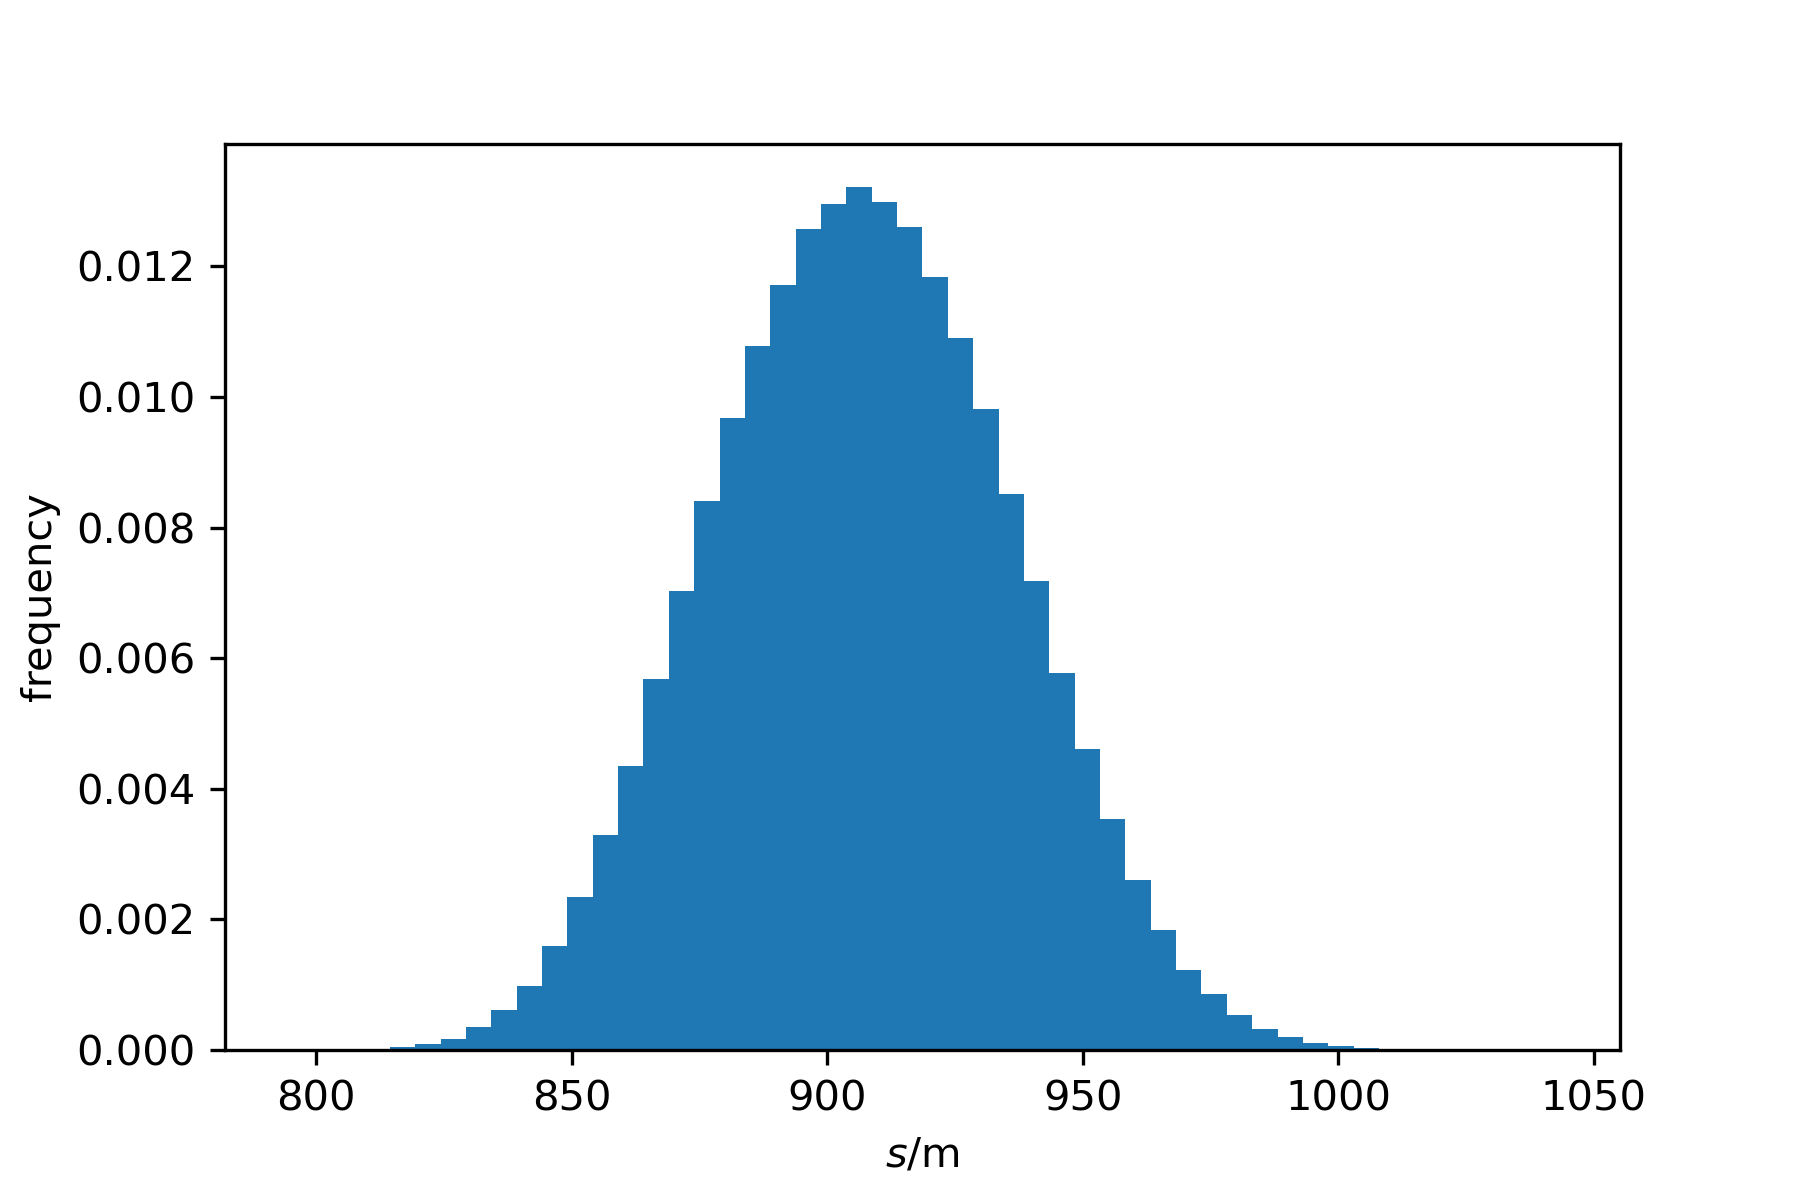
\includegraphics{figures/BrakingDistance.png}

    \begin{tcolorbox}[breakable, size=fbox, boxrule=1pt, pad at break*=1mm,colback=cellbackground, colframe=cellborder]
\prompt{In}{incolor}{ }{\boxspacing}
\begin{Verbatim}[commandchars=\\\{\}]

\end{Verbatim}
\end{tcolorbox}


    % Add a bibliography block to the postdoc
    
    
    
\end{document}
